% \iffalse
\let\negmedspace\undefined
\let\negthickspace\undefined
\documentclass[journal,12pt,twocolumn]{IEEEtran}
\usepackage{cite}
\usepackage{amsmath,amssymb,amsfonts,amsthm}
\usepackage{algorithmic}
\usepackage{graphicx}
\usepackage{textcomp}
\usepackage{xcolor}
\usepackage{txfonts}
\usepackage{listings}
\usepackage{enumitem}
\usepackage{mathtools}
\usepackage{gensymb}
\usepackage{comment}
\usepackage[breaklinks=true]{hyperref}
\usepackage{tkz-euclide} 
\usepackage{listings}
\usepackage{gvv}                                        
\def\inputGnumericTable{}                                 
\usepackage[latin1]{inputenc}                                
\usepackage{color}                                            
\usepackage{array}                                            
\usepackage{longtable}                              
\usepackage{calc}                                             
\usepackage{multirow}                                         
\usepackage{hhline}                                           
\usepackage{ifthen}                                           
\usepackage{lscape}

\newtheorem{theorem}{Theorem}[section]
\newtheorem{problem}{Problem}
\newtheorem{proposition}{Proposition}[section]
\newtheorem{lemma}{Lemma}[section]
\newtheorem{corollary}[theorem]{Corollary}
\newtheorem{example}{Example}[section]
\newtheorem{definition}[problem]{Definition}
\newcommand{\BEQA}{\begin{eqnarray}}
\newcommand{\EEQA}{\end{eqnarray}}
\newcommand{\define}{\stackrel{\triangle}{=}}
\theoremstyle{remark}
\newtheorem{rem}{Remark}
\begin{document}

\bibliographystyle{IEEEtran}
\vspace{3cm}

\title{NCERT DISCRETE}
\author{EE23BTECH11020 - Raghava Ganji$^{*}$% <-this % stops a space
}
\maketitle
\newpage
\bigskip

\renewcommand{\thefigure}{\theenumi}
\renewcommand{\thetable}{\theenumi}

\textbf{Question 10.5.3.5:}
The first term of an AP is $5$, the last term is $45$ and the sum is $400$. Find the number of terms and the common difference.\\
\textbf{solution:}\\
Given AP is 5, \ldots, 45.\\\\
\begin{table}[h]
\centering
\begin{tabular}{|c|c|c|}\hline
$x(0)$ & $5$ & $ 1st\hspace{1mm}term$\\ \hline
$x(n-1)$ & $45$ & $nth\hspace{1mm}term$\\ \hline
$s(n-1)$ & $400$ & $sum\hspace{1mm}of\hspace{1mm}n\hspace{1mm}terms$\\ \hline
$n$ & $?$ & $no.of\hspace{1mm}terms$\\ \hline
$d$ & $?$ & $common\hspace{1mm}difference$\\ \hline
\end{tabular}
\caption{parameters}
\end{table}
\begin{align}
x(n)&=x(0)+nd\\
40&=(n-1)d\\
s(n)&=\frac{n+1}{2} [2x(0)+nd]\\
s(n-1)&=\frac{n}{2} [2x(0)+(n-1)d]\\
n&=16\\
d&=\frac{8}{3}
\end{align}
by substituting the value of n in the equation 2, we get the equation 6.\\
z transform of $x(n),s(n)$ are $X(z),S(z)$
\begin{align}
X(z)=\frac{7}{3(1-z^{-1})}+\frac{8}{3(1-z^{-1})^2}\\
S(z)=\frac{7}{3(1-z^{-1})^2}+\frac{8}{3(1-z^{-1})^3}
\end{align}
\begin{figure}
    \centering
    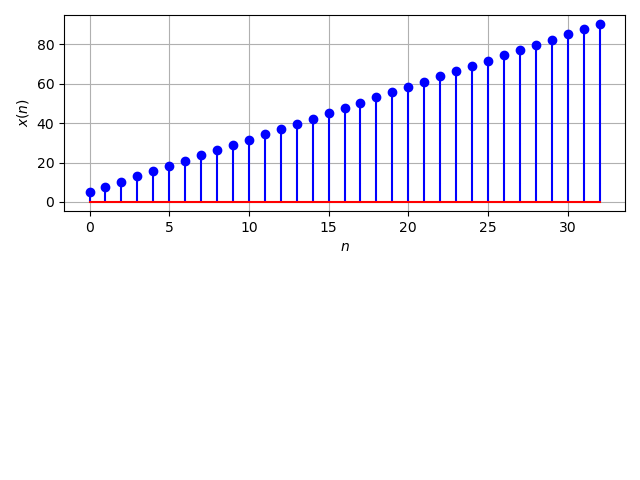
\includegraphics[width=1\linewidth]{1.png}
    \caption{1}
    \label{fig:enter-label}
\end{figure}
\end{document}
